\subsection{Design System}
A design system is typically built for web based products to maintain a consistent user experience across different web based products. In recent years, the topic of design systems has received more and more attention from companies as more and more products move away from on-premises solutions, towards web-based products.  With the help of a central system that provides not only with its components, but also with guidelines and patterns.  \citep{macdonald_practical_2019} \\
Design systems are often compared to component libraries and style guides. This happens because a design system contains the same parts as the other two. It is important to understand that a design system includes both design processes and design philosophy.  It serves as a basis for discussion between product managers, designers and front-end developers.   \cite{vesselov_building_2019} \\
The following definitions of design systems can be found in the literature:
\begin{tcolorbox}[title=Definition of design system by \citet*{macdonald_practical_2019}]
A design system is a single source of truth for shared parts and processes, such as components, patterns, and guidelines, to build consistent products. [...] Additionally, design systems reflect the culture, team values, and visual language of an organization.
\end{tcolorbox}
Another definition goes even further and specifies the aspect of documentation of design systems:
\begin{tcolorbox}[title=Definition of design system by \citet*{vesselov_building_2019}]
A series of documented elements, components, and regions that include both design and front-end guidelines. The documentation contains live code examples, allowing cross-functional teams to easily reuse styles and components in several instances across an application. A design system also includes underlying design principles, rules, and guidelines that help a team build one or multiple products.
\end{tcolorbox}
A basic structure of design systems can be derived from both definitions. According to this, a design system can be divided into three different parts. On the one hand, there are the guidelines, which provide users with instructions on how to use the design system and build how to build the software product. As a further subdivision are the components, which a developers or designers use. These must be made available as simple as possible so that they can be easily integrated into the end product. The last and most underestimated part is the documentation mentioned by \citet*{vesselov_building_2019}. The best components can be provided, but without clear and interactive documentation, they are only half as good.  These sections will be discussed further in the remainder of this chapter. \cite{macdonald_practical_2019}\cite{vesselov_building_2019}

\subsubsection{Guidelines}
Guidelines are an important part of a design system to differentiate from a component library. Of course, component libraries also have guidelines to ensure that developers use them correctly, but these are technical in nature.  \\
Guidelines in Design systems are to serve as communication assistance between designers and all other involved ones. The manual effort of handoffs between UX and the development team can be handled more efficiently. Many issues can be addressed up front with well thought out guidelines, giving developers and designers more time to do their jobs. In case there are still open design questions, the guidelines from the design system serve as a basis for discussion. \cite{vesselov_building_2019} \\
It is important to mention that guidelines are not static images and long texts. They must automatically grow with the design system and be well structured. At best, a design system is structured so that the listed components document themselves. A good structure also includes a user-friendly navigation, which allows to find and search for components or documentation of any kind in the design system. This is supported for example by autocomplete searches, overview pages and tables of contents.  \cite{macdonald_practical_2019}\cite{vesselov_building_2019} \\
As in the usual software development of large projects, it is common to apply versioning. Also in design systems it is important to have versioning not only in the code, but also in the documentation and guidelines. This way it is possible to track changes to policies and implement them correctly for the version used by the developer. Speaking of large projects, an issue tracker should also be used in design systems, which allows reporting bugs and improvements. Furthermore, release notes with detailed description by image and text help to motivate users to follow the design system and stay up to date. This makes updating to new versions as convenient as possible for the developers. \cite{macdonald_practical_2019} \\
But it's not just developers who benefit from the guidelines. For example, a product manager may have an idea for a new feature that he wants to present to customers. However, the UX team doesn't have the resources to mock up the idea on the fly. The guidelines still allow the product manager to create a proof-of-concept within the given capabilities and present it to the customer. Properly applied, the product manager can be confident of meeting UX requirements.  \cite{vesselov_building_2019} \\
Another use case for guidelines in a design system are onboarding processes within companies. Both the above-mentioned developer and product manager can use the guidelines to find their way around the product faster, but people from sales or marketing can also use this resource.  In the literature, these guidelines are also referred to as a common design language for a company.  \\
According to \citet*{vesselov_building_2019}, guidelines can be divided into four different types: 

\paragraph*{Formal definition} 
Description of a component and its function. For the developer the documentation may seem trivial, but it helps to avoid misunderstandings. \cite{vesselov_building_2019}
\begin{figure}[htbp]
\centerline{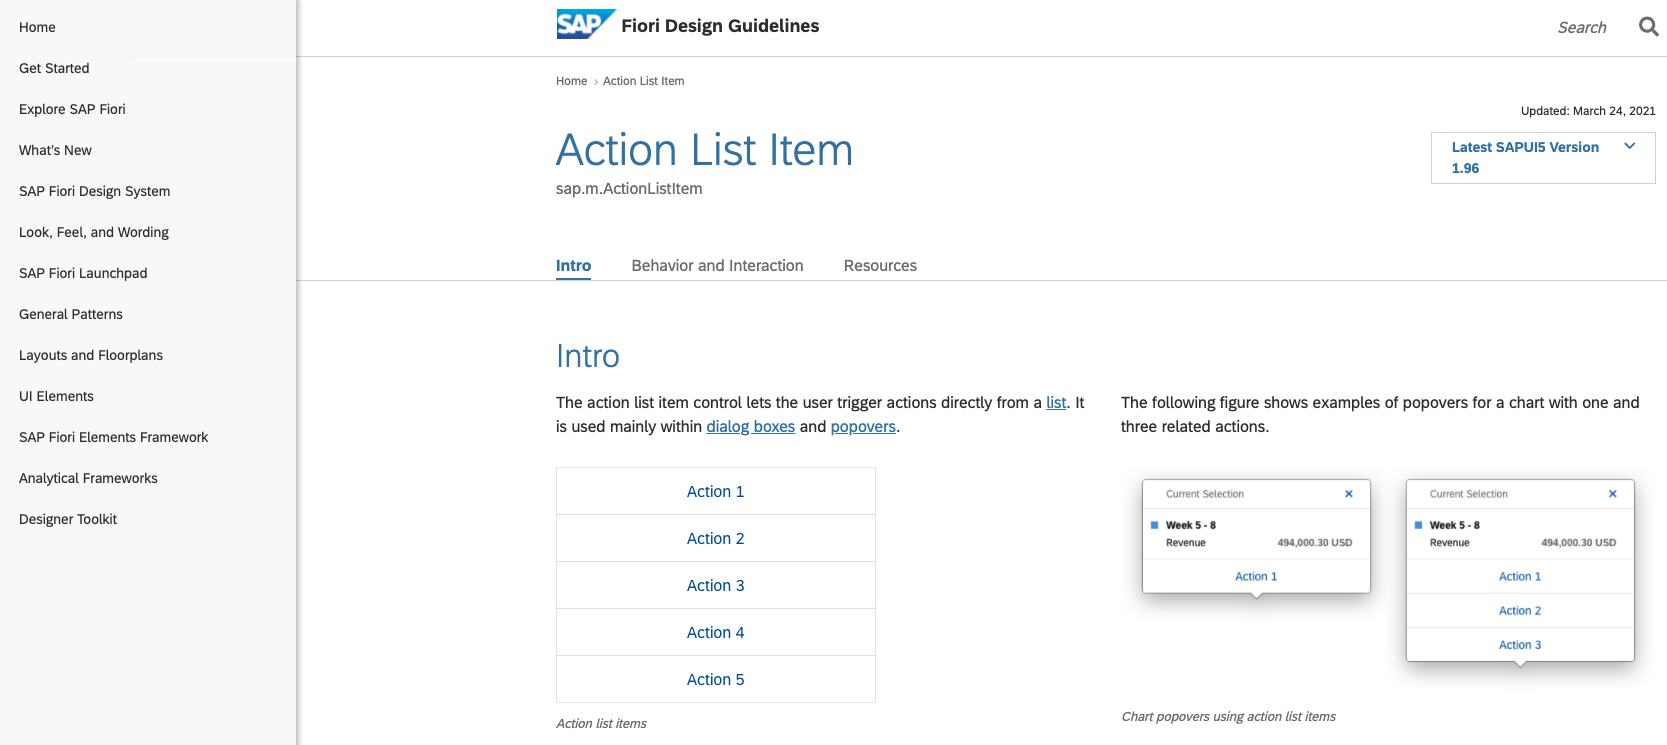
\includegraphics[width=\linewidth]{images/fiori_action-list_formal.png}}
\caption{SAP Fiori Action List formal guideline \cite{sap_fiori_action_nodate}}
\label{fiori_action_list}
\end{figure}
\paragraph*{Usage guidelines} Here the questions should be clarified how to use the components. Furthermore, the parameters and their use are explained. The user should know from this documentation how to configure and use the component. \cite{vesselov_building_2019}
\begin{figure}[htbp]
\centerline{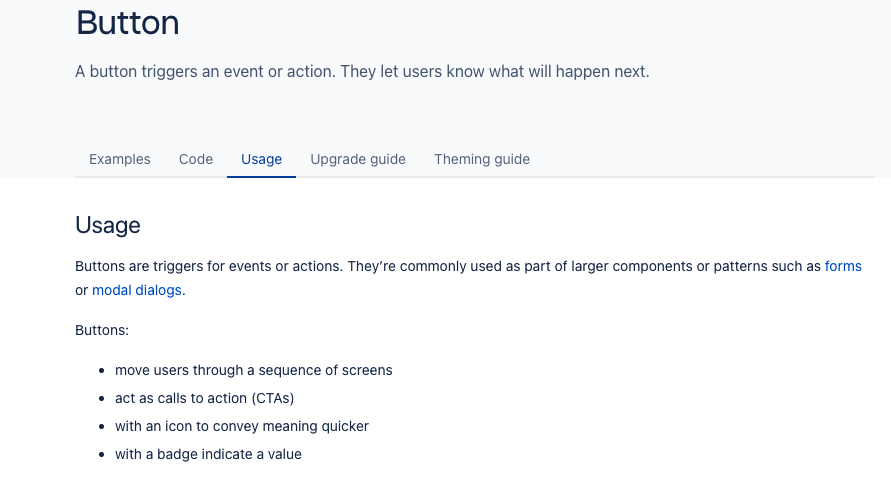
\includegraphics[width=\linewidth]{images/atlassian_button_usage.png}}
\caption{Atlassian Design System Button usage guideline \cite{atlassian_button_nodate}}
\label{fiori_action_list}
\end{figure}
\paragraph*{Technical guidelines} \label{tech_guideline}
This part of the guide is mainly intended for developers who are to implement the documented component in the software. Any ambiguities about the implementation should be clarified here. Also how the presented parameters can be used to configure the component. An often found feature here is copying code snippets. This allows developers to immediately copy-paste the component code they have just read into their code.  \cite{macdonald_practical_2019} \cite{vesselov_building_2019}
\begin{figure}[htbp]
\centerline{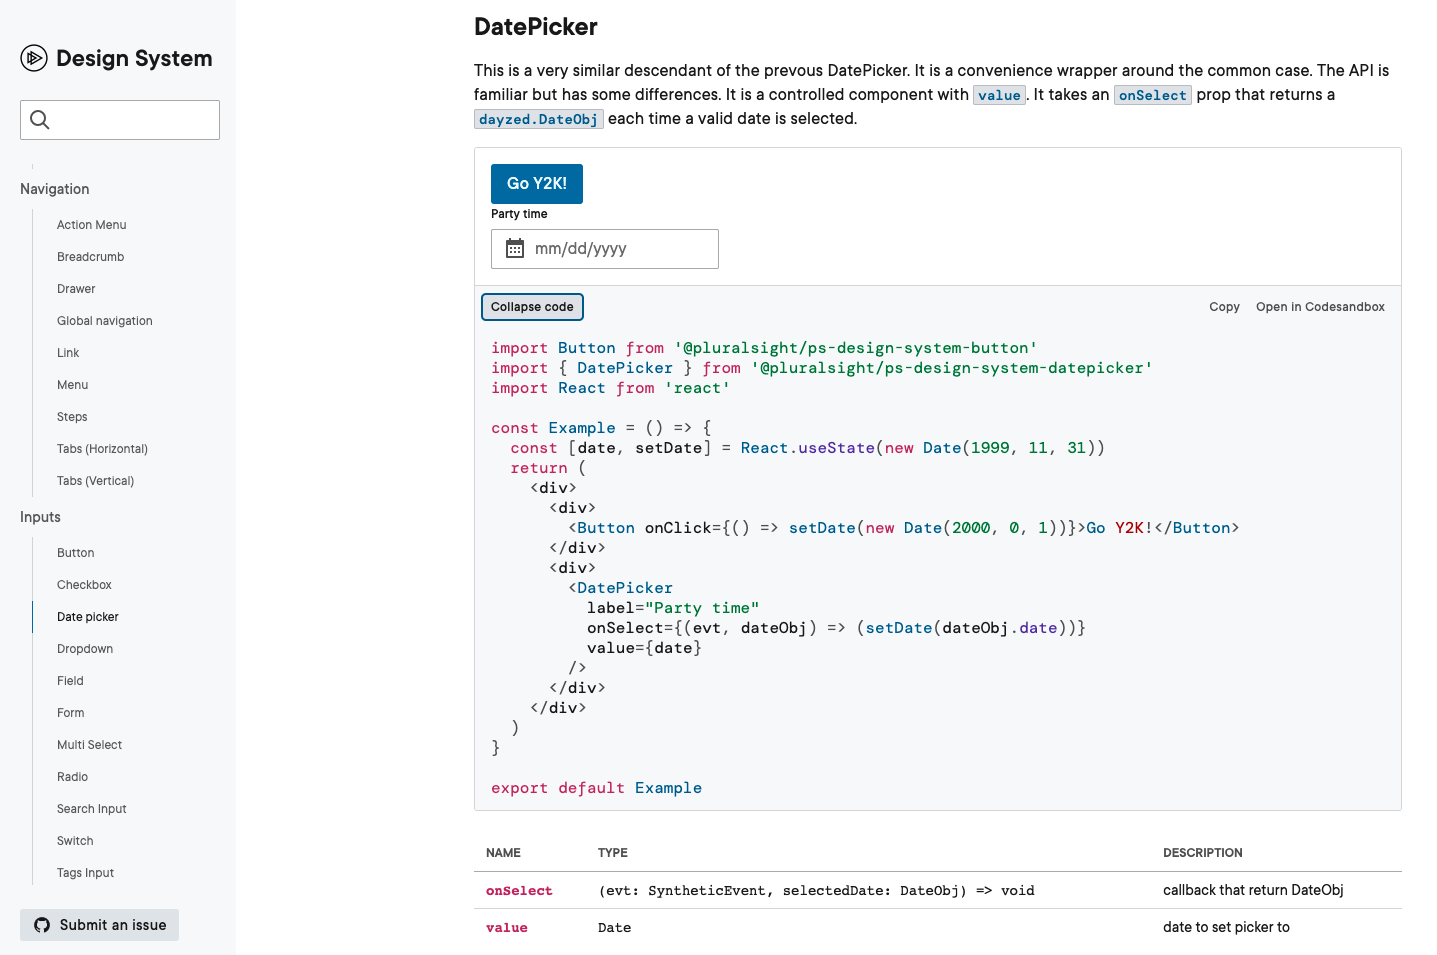
\includegraphics[width=\linewidth]{images/pluralsight_date-picker_technical.png}}
\caption{Pluralsight Design System Date picker technical guidelines \cite{pluralsight_datepicker_nodate}}
\label{fiori_action_list}
\end{figure}
\paragraph*{Related components} Linking components and regions help the user explore the design system. Also, this can help the creative process for designers and developers.  \cite{vesselov_building_2019}
\begin{figure}[htbp]
\centerline{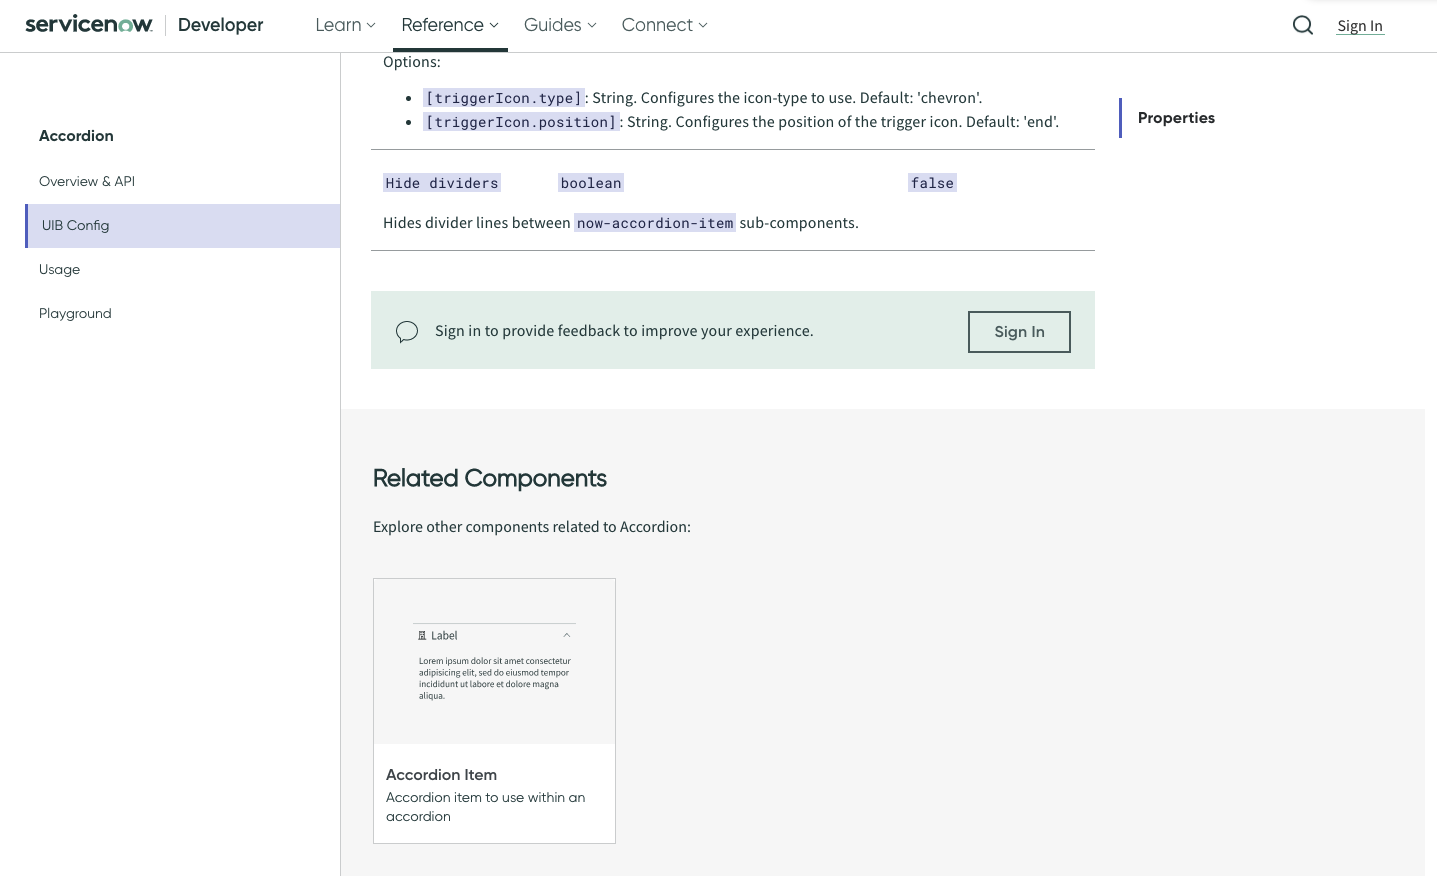
\includegraphics[width=\linewidth]{images/servicenow_accordion_related.png}}
\caption{Servicenow Accordion related components \cite{servicenow_now_nodate}}
\label{fiori_action_list}
\end{figure}

\subsubsection{Design Principles}
Design principles should be a central consideration when building a design system. In doing so, design principles should reflect the norms and values of the product organization.  In doing so, the points established do not follow any rules, except that they are established collectively by the team.  \\
Thus, these design principles serve as a basis for discussion and decision-making for designs. By simply self-explanatory principles it is possible for the designers and developers to quickly create new designs without a large coordination effort. Often questions are taken as principles. This gives developers and designer an impulses to ask themselves if they are aligned with the design principles during the creation process. \cite{brignell_design_2022} \\
As an example there are design principles for the Web by \citet{berners-lee_principles_2013}: 
\begin{itemize}
\item \textbf{Simplicity} - Simple solutions are better solutions
\item \textbf{Modular Design} - Change things and it will only affect one part
\item \textbf{Being part of a Modular Design} - Realize you own the Design System
\item \textbf{Tolerance} - "Be liberal in what you require but conservative in what you do"
\item \textbf{Decentralization} - Don't produce bottlenecks, allow scaling in any direction
\item \textbf{Test of Independent Invention} - "Designing a system not to be modular in itself, but to be a part of an as-yet unspecified larger system."
\item \textbf{Principle of Least Power} - Use matching tools for the matching tasks
\end{itemize}
Design principles can be quite different. In this case, they are relatively technical, as the team wants to focus on these issues. Other organizations, such as Adobe (\url{https://spectrum.adobe.com/page/principles/}), have people at the forefront.  \\
The design principles play a central role in a design system. The importance these anchor points is often underestimated. The product team should not only build software based on these principles, but also gain an understanding of the big picture of the product organization. Thus, design principles should be aligned with the design strategy of the company.  In this way, not only is the existing product organization aligned with the design principles, but new employees can also use them to more quickly integrate themselves into the product organization.  Design principles are effective when they serve as a guide for the creative process.\cite{vesselov_building_2019} \\
In order to apply design principles, they must first be created. While it would be possible to create them yourself, it is not recommended because these principles are intended to reflect the creative thinking of a large group of the product organization. Here, \citet{vesselov_building_2019} lay out a 5-step plan to iteratively create and continuously improve them. In the following figure \ref{design_principles_steps}, these 5 steps can be seen:
\newpage


\begin{figure}[htbp]
\centerline{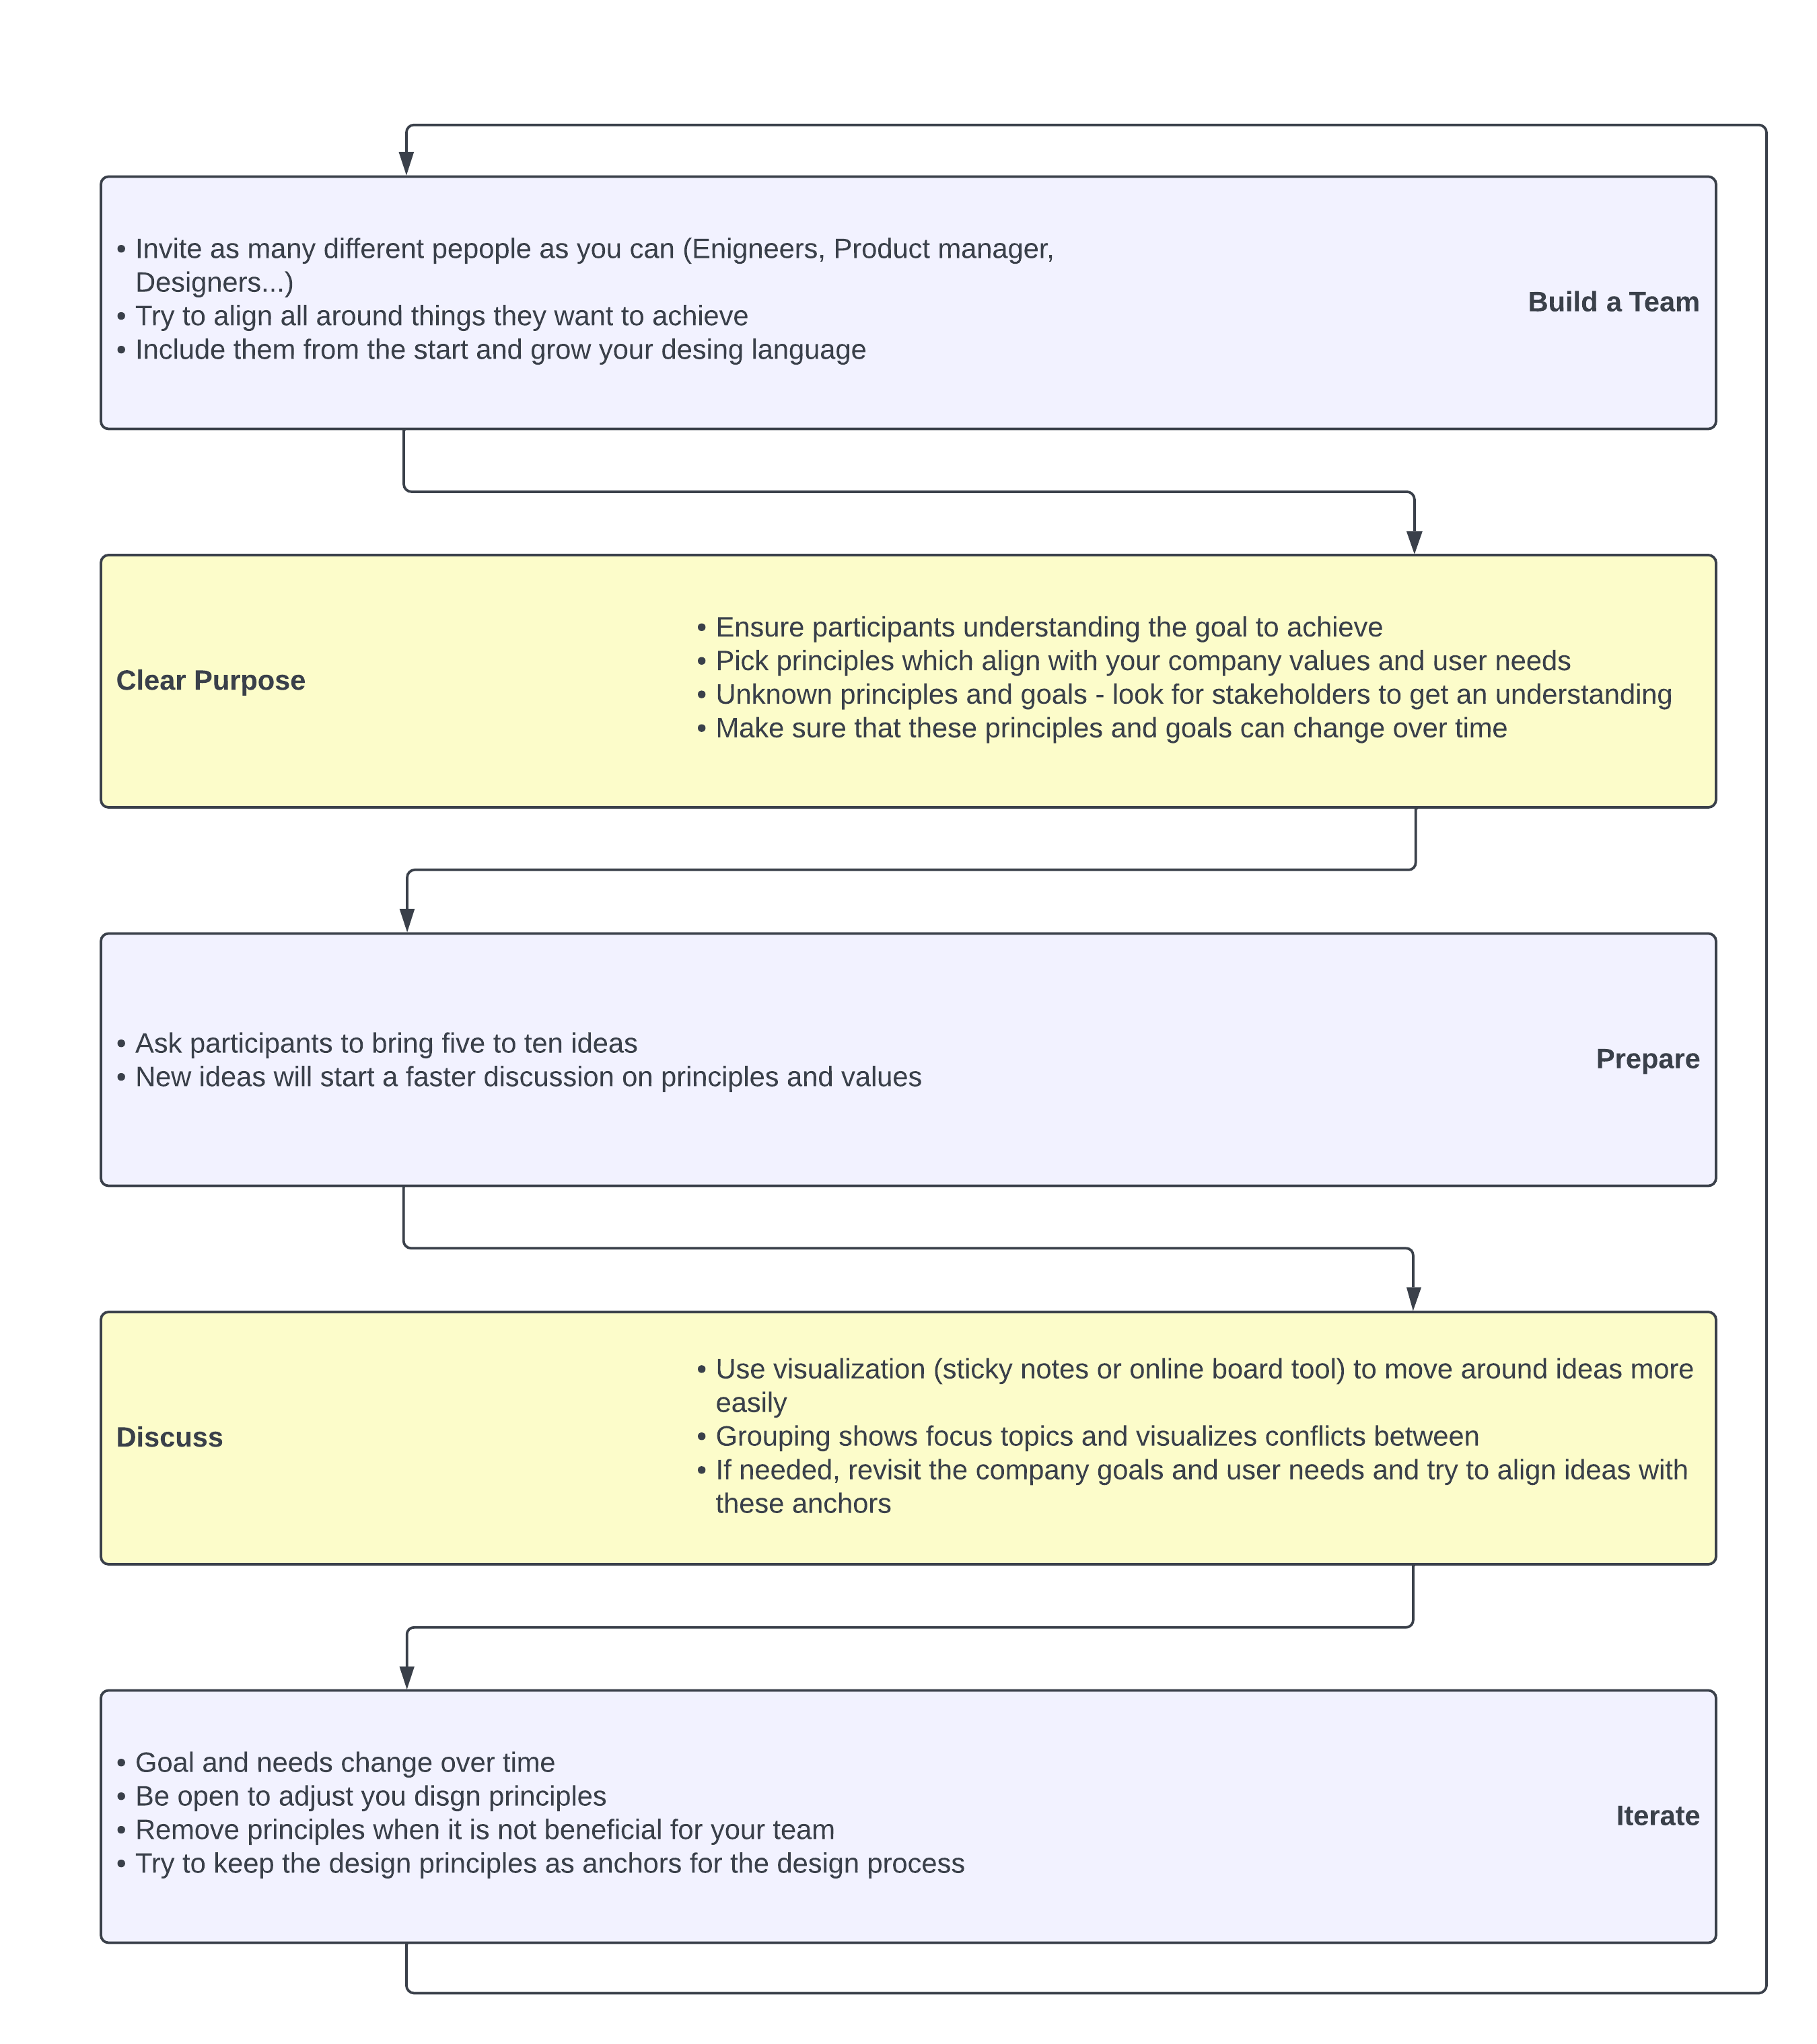
\includegraphics[width=\linewidth]{images/design_principles_steps.png}}
\caption{5 steps to introduce design principles inspired by  \citet{vesselov_building_2019}}
\label{design_principles_steps}
\end{figure}
Once design principles are in place and an iterative process to keep them up to date is installed, there is a need to share these principles with the rest of the product organization. This is where many design systems offer what are called design blogs or design news. They not only help the organization keep track of the design principles in their daily work. They also provide a platform to share updates with users.  Moreover, there is an exchange on related topics on these platforms. This in turn helps to improve and keep the design system and design principles up to date.  \cite{google_material_2022}\\

Having set the foundation with the guidelines and design principles, the next chapter will deal with another important building block, the component library.
\subsubsection{Component Library}
The technical counterpart to the description guidelines and design principles is the component library. Both cannot exist in a design system without each other.  By definition, a component is "a constituent part" \cite{component_definition} of in this case a user interface.  Combined with library, which means a "collection of something"\cite{library_definition}, it results in a collection of important constituent parts for user interfaces.  \\
The definitions existing from the literature are as follows:
\begin{tcolorbox}[title=Definition of component library by \citet*{vesselov_building_2019}]
A set of styles and components that can be used and shared among a team. A component library consists of common core elements that are used throughout an application. [...] Component libraries may or may not include living code. [...] Unlike UI frameworks such as Bootstrap, component libraries are tailored to specific purposes, like an internal brand.
\end{tcolorbox}
In addition to components, there are also styling rules that also include layout specifications in component libraries. 
\begin{tcolorbox}[title=Definition of component library by \citet*{macdonald_practical_2019}]
Component libraries, UI libraries, or code libraries provide frontend code for UI components (a.k.a. widgets, modules, chunks, blocks). Internally, you might use a component library as a shared collection of UI snippets implementing patterns that anyone in the organization can contribute to building.
\end{tcolorbox}
An important point that emerges from these definitions is that component libraries have a clear focus on internal use. This is also the main difference to UI frameworks. \\
After reviewing various design systems, their component libraries can be split into the following 4 points:
\begin{itemize}
	\item \textbf{Layout} - Spacing and presentation of content placement on a site
	\item \textbf{Styles} - Color definitions, Typography, Icons
	\item \textbf{Components} - Reusable parts fulfilling one purpose
	\item \textbf{Regions} - Combination of multiple components 
\end{itemize}




% Six interlocking areas make up a design system: layout, styles, components, regions, content, and usability. A robust design system should contain guiding design principles, guidelines for use and implementation, as well as a component library that includes front-end code. \cite[p.23]{vesselov_building_2019}

% Vesselov ab Seite 71
% https://design-system.service.gov.uk/
% Wie GOV AUS 

% https://www.bbc.co.uk/gel
% Kein Komponenten sondern Fokus auf Patterns, Foundation als Principles
\paragraph{Layout}
The foundation of any design system is the ability to place, move, or arrange elements on web pages. To achieve a consistent appearance, it is important to align spacing and positioning. 
For this purpose, so-called design tokens in the form of CSS variables are often used. Similar to Tailwind (\url{https://tailwindcss.com/}), these variables are then translated into CSS classes so that the developer does not have to use the variables natively. And thus does not need to know CSS.  \\
Salesforce Lightning Design System, for example, lists all layout tools under "Utilities." It sets sizes for text, simple boxes, and spacing between components. In fact, a sophisticated grid layout system can be seen as well. \\

IMAGE

As can be seen, CSS classes are used to achieve the desired layout. Both dynamic and static layouting are supported. So the user has all the possibilities to use the layout of the design system. \\
Besides the usual regulations for spacing and positioning, other points like visibility, scrollability or printability can also be described in the layout. Basically, all requirements for visible elements in the target system can be specified by the default layouting in the design system.

\paragraph{Styles}
Styles are about colors, typography and icons. Here it is important to establish a connection to the chosen design principles. This helps to better convey the overall design language in the next steps. 
It is important to mention that when using the style theme in multiple products, there should be a possibility to configure it. This way, each product can still have a unique look and feel. \cite{vesselov_building_2019}
\subparagraph{Color}
The introduction of a color system is a good first step on the way to a design system. Colors are important for the aesthetics of a product and can be easily iterated and changed without changing functionality or layout. It is always important to keep accessibility in mind when choosing colors. For certain text sizes, it is important to maintain a certain contrast. The WCAG (\url{https://www.w3.org/WAI/standards-guidelines/wcag/}) describes this contrast with two levels AA and AAA. This contrast is especially important if the product has several long paragraphs.  \\
Usually, not a single color is created, but an entire palette. The colors are often divided into primary, secondary, text color, background color, accent colors, shadows and so on. Also here CSS variables with the appropriate names are created to use them. The challenge is to offer a well-defined color palette, but at the same time not to overload the user, because with too many colors the overview gets lost quickly. \cite{vesselov_building_2019}


IMAGE 


\subparagraph{Typography}
When it comes to a typography system, it can be divided into two categories of typography. First, there is typography that is used for two or perhaps three words at a time, such as headings or button elements. Second, there is defined typography for longer texts such as paragraphs. \\
In both cases, it must follow the defined layout system. Important things like baseline height, padding, and margins are important here. A helpful piece of advice is to represent all types of text possibilities in your typography system.  \cite{vesselov_building_2019}


IMAGE

\subparagraph{Iconography}
There is no need to create iconography with each new design system. In the wild, there are many good options that can be used right away. But creating a new iconography provides many opportunities to visualize your own design language in the iconography.
\\
As with other parts of a design system, documentation is key. How to create new icons, what proportions and shapes are important. If done right, it's an easy step to introduce new icons into the iconography. 
\\
To make them accessible to the team, there should be a description of how to add them to the software. There should be the same representation of the source code as in the technical guidelines in \ref{tech_guideline}. \cite{vesselov_building_2019}


IMAGE
\paragraph{Components}
With all the tools and fundamentals in hand, the main part of a component library, the components can be assembled. Components should be highly reusable and as flexible as possible. They represent building blocks of applications.  \\
From combinations of layout and style specifications components emerge for different use cases. By using these defined components within applications, the developer ensures that guidelines are followed. For certain combinations of components in an application, there is another term called regions, which is explained in more detail in the next chapter \ref{regions}. \\


EXAMPLE OF COMPONENT


DOCUMENTATION EXAMPLE


In order to achieve flexibility and reusability, it is important to have always the interfaces of the component in the mind. Well defined interfaces are the key to successful components. To achieve this, always involve the engineers building the actual product to get their feedback on the interfaces. As with other parts of a design system, documentation is key. A well-structured and systematic approach to how a component works helps developers use the components.  \cite{vesselov_building_2019}



INTERFACE EXAMPLE
\paragraph{Regions} \label{regions}
Often, a combination of certain components is used over and over again in different places and even in different applications. To cover this use case, a design system has a concept called regions. Regions specify a combination of several components and document the use and composition of these components. They can be seen as an extended documentation to reproduce a certain behavior in an application. 
\\
Regions refer not only to the interaction of components, but also to the switching of visualization due to changes in a user's permissions, for example. All these types of UI-related documentation needed to define a particular user experience can be documented here.   \cite{vesselov_building_2019}
\\
Most often, regions appear in the general navigation of applications. They evolve naturally from the finished products and grow iteratively with more and more feedback from the product development team.
\\
A good example is the navigation bar. Components such as buttons and dropdown components can be used in combination with the skeleton of a navigation bar to create the region called Navigation Bar. 
